%%%%%%%%%%%%%%%%%%%%%%%%%%%%%%%%%%%%%%%%%
% Original author:
% Linux and Unix Users Group at Virginia Tech Wiki
% (https://vtluug.org/wiki/Example_LaTeX_chem_lab_report)
% Modified by: Hector F. Jimenez S, for the Digital Electronics Laboratory.
% License:
% CC BY-NC-SA 3.0 
%%%%%%%%%%%%%%%%%%%%%%%%%%%%%%%%%%%%%%%%%
%----------------------------------------
%	PACKAGES AND DOCUMENT CONFIGURATIONS
%---------------------------------------
\documentclass[paper=a4, fontsize=12pt]{article} 		% A4 paper and 11pt font size
\usepackage[T1]{fontenc} 								% Use 8-bit encoding that has 256 glyphs
%\usepackage{fourier}		 							% Use the Adobe Utopia font for the document 
\usepackage[spanish,english]{babel}						% Spanish Language, templates uses some sections in english.
\selectlanguage{spanish}								% main language.
\usepackage{subfig}
\usepackage{multirow}
\PassOptionsToPackage{spanish}{babel}
\renewcommand{\figurename}{Figura}						% Force rename of figure.
\renewcommand{\figurename}{Fig.}
\usepackage[figurename=Fig.]{caption}
\usepackage[utf8]{inputenc}								% tildes for spanish language.
\usepackage{amsmath,amsfonts,amsthm} 					% Math packages.
\usepackage{minted}										% For syntax highlighting.
	    \renewcommand\listingscaption{Código}			%rename the source code minted !
\usepackage{float}										% Image will be in the same place as you want.!!! x-/
\usepackage{sectsty} 									% Allows customizing section commands
\allsectionsfont{\centering \normalfont\scshape}	   	% Make all sections centered, the default font and small caps
\usepackage{hyperref}
\hypersetup{											%Setups the false color and borders.
    colorlinks=false,
    pdfborder={0 0 0},
}
\newcommand\fnurl[2]{%									% set a simple and quick footnote command and include url.
\href{#2}{#1}\footnote{\url{#2}}%	
}
\usepackage{graphicx}									% Import easyly images.
\graphicspath{ {./images/} }							% Where to look for the images.
\DeclareGraphicsExtensions{.pdf,.png,.jpg}				% Graphics Extension to be used
\usepackage[notes,backend=biber]{biblatex-chicago}		% Bibliography and references.
\bibliography{biblio}									% bibliography filename.
\usepackage{fancyhdr} 									% Custom headers and footers
\pagestyle{fancyplain} 									% Makes all pages in the document conform to the custom headers and footers
\fancyhead{} 											% No page header
\fancyfoot[L]{} 										% Empty left footer
\fancyfoot[C]{} 										% Empty center footer
\fancyfoot[R]{\thepage} 								% Page numbering for right footer
\renewcommand{\headrulewidth}{0pt} 						% Remove header underlines
\renewcommand{\footrulewidth}{0pt} 						% Remove footer underlines
\setlength{\headheight}{13.6pt} 					    % Customize the height of the header
\numberwithin{equation}{section}						% Number equations within sections (i.e. 1.1, 1.2, 2.1, 2.2 instead of 1, 2, 3, 4)
%\numberwithin{figure}{section} 						% Number figures within sections (i.e. 1.1, 1.2, 2.1, 2.2 instead of 1, 2)
\numberwithin{table}{section} 							% Number tables within sections (i.e. 1.1, 1.2, 2.1, 2.2 instead of 1, 2, 3, 4)
\setlength\parindent{0pt} 								% Removes all indentation from paragraphs
\newcommand{\horrule}[1]{\rule{\linewidth}{#1}} 		% Create horizontal rule command with 1 argument of height
\usepackage{listings}% http://ctan.org/pkg/listings
\usepackage{multicol}
\usepackage{caption}
\usepackage{subfig}
\renewcommand{\lstlistingname}{Código}	
\title{Sistemas Operativos I\\ 
\horrule{0.5pt} \\[0.4cm] 								% Thin top horizontal rule	Title rule
\textit{Taller 3: Caso de estudio del sistema operativo MSDOS6.22, exploración superficial}
\horrule{1pt} \\[0.5cm] 			
} 			

\author{												
Héctor F. \textsc{Jiménez Saldarriaga.}\\				% Authors begin.
\texttt{hfjimenez@utp.edu.co} \\						
\texttt{PGP KEY ID: 0xB05AD7B8}
} 
% End of  Author name
\date{}    						                       % Date for the report, this will hide the \today.

\begin{document}
\maketitle                      			           % Insert the title, author and date
\begin{center}
\begin{tabular}{l r}								   % two column to
Fecha de Entrega: & Marzo, 2018 \\				   % Ramiro's Details.
Profesor: & Cesar Manuel Castillo Rodriguez
\end{tabular}
\end{center}
%%%%%%%%%%%	
% Let's start the document.
%%%%%%%%%%%	
\section{Objetivos}
\begin{itemize}
	\item Realizar el proceso de instalación del sistema operativo
	\item Identificar Comandos 
    \item Identificar el manejo de Archivos, Shell
    \item Practicar y ejecutar 25 comandos de su selección y presentando el resultado de su ejecución.
	\item Crear un archivo de texto utilizando el comando “Edit” y mostrar el resultado.
\end{itemize}
\section{Proceso de instalación MSDOS 6.22 }
Para realizar el proceso de instalación de un sistema operativo MSDOS en su version 6.22 este estilo las personas debían poseer en su poder al menos tres partes:
\begin{itemize}
\item Manual de instalación, aproximadamente 200paginas
\item Disketes
\item Computadora con los requerimientos de la figura \ref{fig:requerimientos}.
\end{itemize}

\begin{figure}[H]
 	\centering
   	\subfloat[Requerimientos de hardware para la instalación, fuente WinWorldPc]{\label{fig:requerimientos}{
   		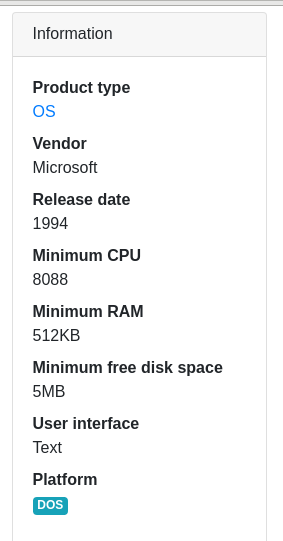
\includegraphics[scale=0.4]{img/requirements.png}}}
\end{figure}
Para realizar la instalación, se realiza un seguimiento detallado de los pasos indicados durante el install wizard,
inicialmente la maquina dará un mensaje de bienvenida (ver figura \ref{fig:bienvenida}), después el instalador preguntara si desea dar formato al disco presente en la instalación e inicia la formateada de este (ver figura \ref{fig:formateada}), para este caso usamos un disco duro de 500MB que es la opción por defecto establecida por Virtualbox. Seleccionamos nuestro teclado y ubicación, en este caso al no existir Colombia, seleccionamos una opción de habla hispana (ver figura \ref{fig:idioma}). Finalmente nuestro archivos quedara ubicados en una particion C:\ y el instalador enviara los archivos allí piden en un orden ascendente los floppy drives de dos6.22. 
\begin{figure}[H]
 	\centering
   	\subfloat[Bienvenida Instalador]{\label{fig:bienvenida}{
   		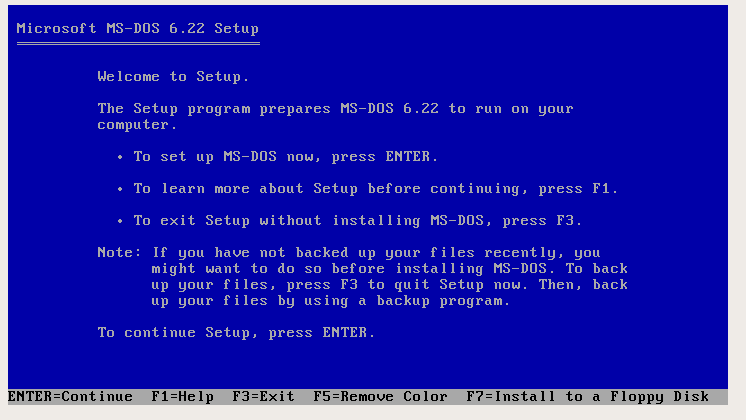
\includegraphics[width=0.68\textwidth]{img/1.png}
   		}}
	\subfloat[Formateado de disco en progreso.]{\label{fig:formateada}{
   		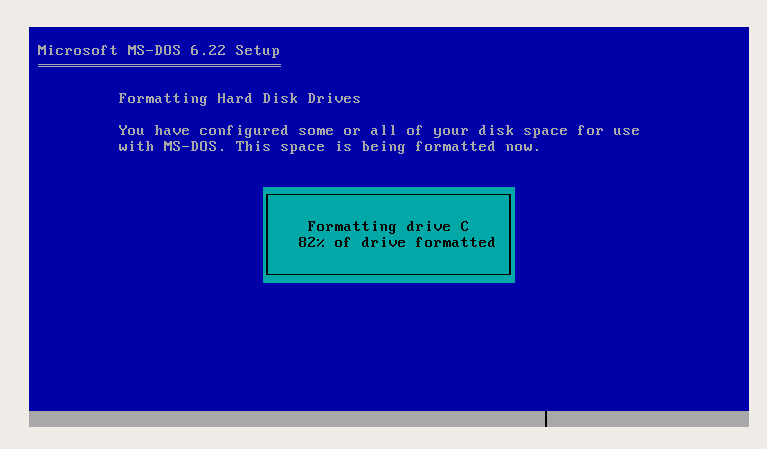
\includegraphics[width=0.68\textwidth]{img/2.png}
        }}
       \hfill
	\subfloat[Seleccion de Idioma.]{\label{fig:idioma}{
   		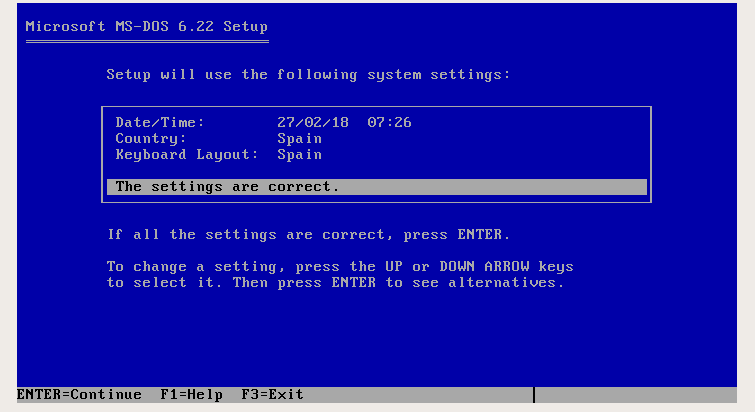
\includegraphics[width=0.68\textwidth]{img/3.png}
        }}
	\subfloat[Selección de ubicación archivos MSDOS.]{\label{fig:ubicacion}{
   		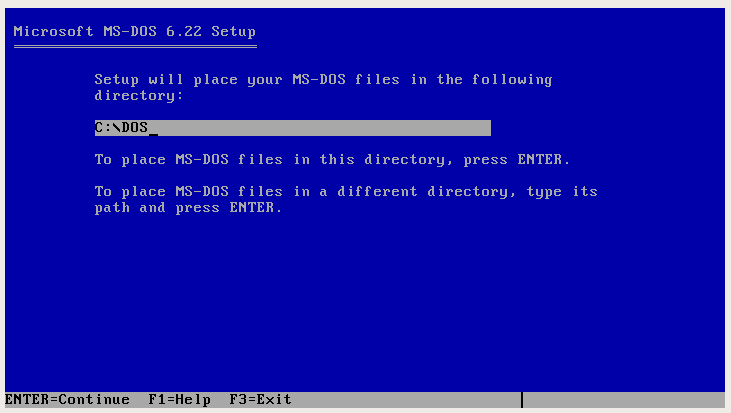
\includegraphics[width=0.68\textwidth]{img/4.png}
        }}
        \hfill
	\subfloat[Instalacion parte 1,2.]{\label{fig:part1}{
   		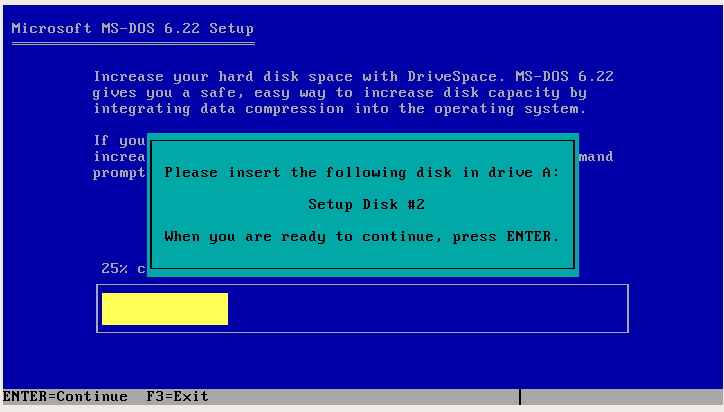
\includegraphics[width=0.68\textwidth]{img/5.png}
        }}
	\subfloat[Instalacion parte 3.]{\label{fig:part2}{
   		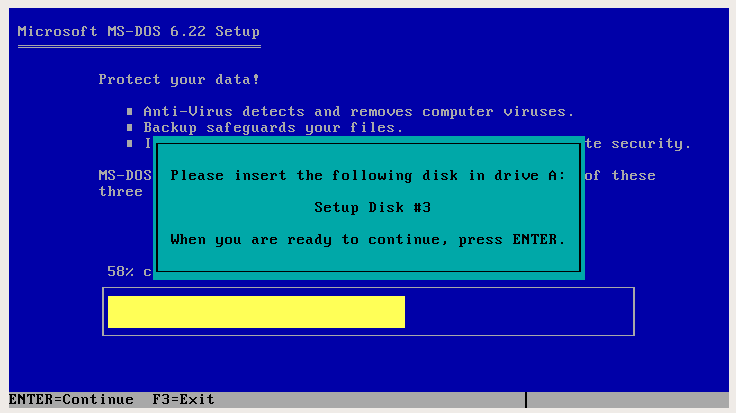
\includegraphics[width=0.68\textwidth]{img/6.png}
        }}
        \hfill
	\subfloat[Instalacion terminada, retiro de floppy drives.]{\label{fig:hecho}{
   		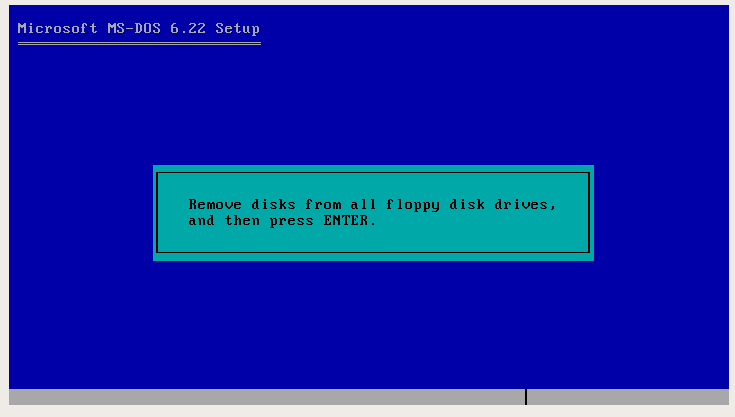
\includegraphics[width=0.68\textwidth]{img/7.png}
        }}
	\subfloat[Finalizacion  de instalación del Sistema Operativo. Comando de instalación de opciones.]{\label{fig:terminado}{
   		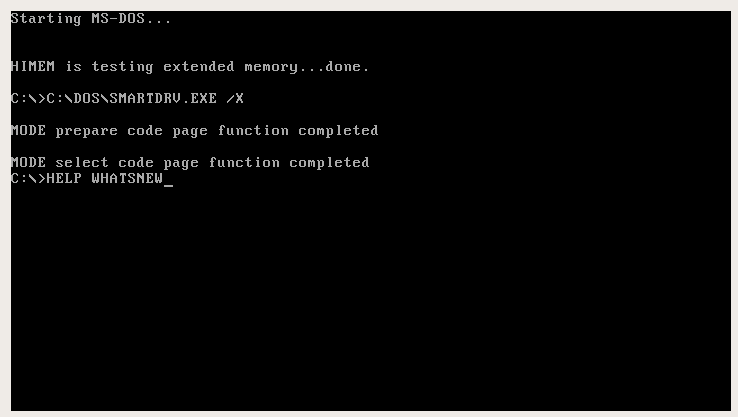
\includegraphics[width=0.68\textwidth]{img/8.png}
        }}
	\caption{Instalación de MSDOS6.22, Virtualbox}
\end{figure}
Una vez tenemos nuestro entorno de sistema operativo funcionando correctamente, es ahora necesario ver las opciones  de ayuda como se presentan, tal cual lo sugeria el sistema operativo en su instalación es posible ver una lista de novedades con el comando de la figura \ref{fig:sugerencia}
\begin{figure}[H]
 	\centering
	\subfloat[Ejecucion comando \textbf{HELP WHATSNEW}]{\label{fig:sugerencia}{
   		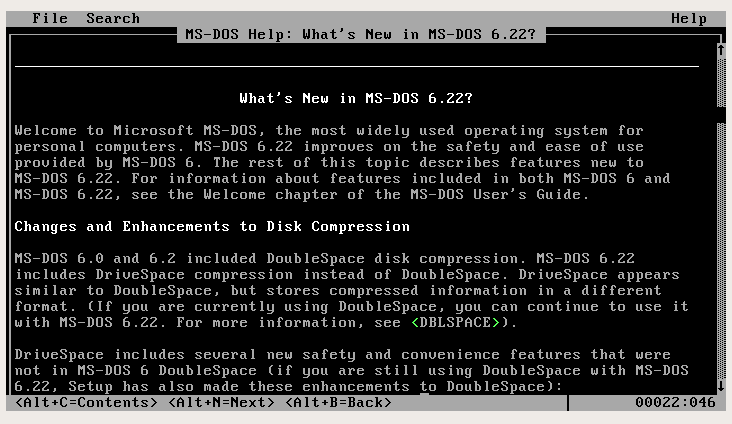
\includegraphics[width=0.68\textwidth]{img/9.png}
        }}
        \hfill
        \subfloat[Ayuda del sistema operativo ]{\label{fig:sugerencia}{
   		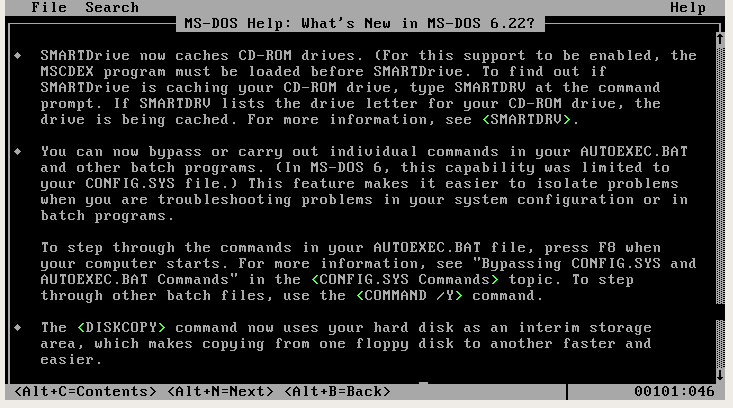
\includegraphics[width=0.68\textwidth]{img/11.png}
        }}
        \subfloat[Listado de comandos disponibles]{\label{fig:disponibles}{
   		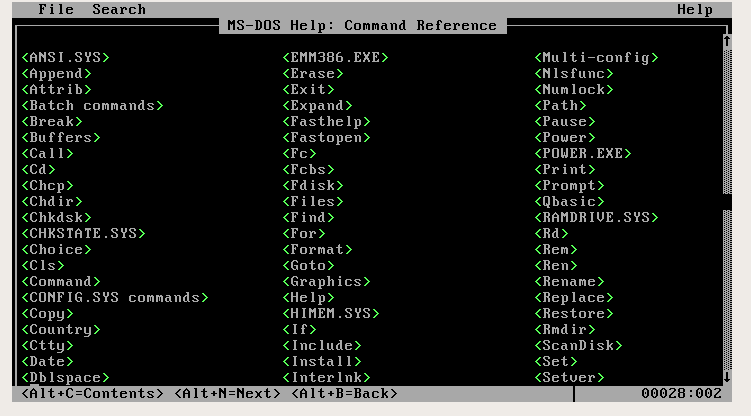
\includegraphics[width=0.68\textwidth]{img/12.png}
        }}
	\caption{Lista de Novedades, Comandos disponibles MSDOS.}
\end{figure}
\section{ Identificación de  Comandos }
Como se menciona en la figura \ref{fig:disponibles} tenemos una  lista de  comandos disponibles, los comandos necesarios permiten que el operador realice ciertas acciones de  diferentes  tipos en el sistema como  :  

\begin{itemize}
\item administración de archivos
\item comandos del sistema 
\item comandos de red
\end{itemize}

\begin{figure}[H]
 	\centering
	\subfloat[Ejecucion comando \textbf{HELP WHATSNEW}]{\label{fig:sugerencia}{
   		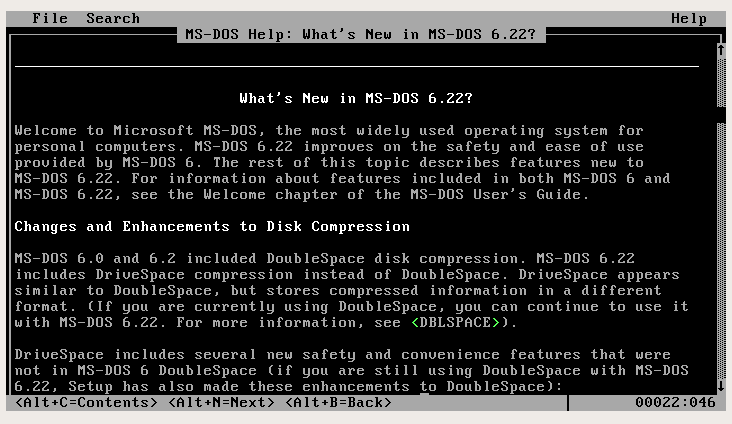
\includegraphics[width=0.68\textwidth]{img/9.png}
        }}
\end{figure}

\section{ Manejo de Archivos}
Como se menciona en la ayuda de whatsnew el sistema de manejo de archivos de msdos6.22 utiliza fat16. En este sistema de archivos los archivos pueden ser de dos tipos:
\begin{enumerate}
\item Directorios regulares
\item Archivos regulares 
\end{enumerate}
Los directorios permiten contener y organizar otros archivos, directorios y los archivos regulares suelen normalmente ser de dos tipos: 
\begin{enumerate}
\item archivos ejecutables, que tienen extensión COM, EXE, BAT. 
\item archivos de datos, contienen información de cualquier tipo, como música formato MIDI imágenes, entre otros.
\end{enumerate}
Los archivos ejecutables son procesados por una función global que se encarga a leer el archivo revisando los headers de este, el sistema operativo verificará 
\section{ Ejecución de comandos .}
Para realizar esta sección se realiza la ejecución de los 25 comandos, se juega con varios de ellos de manera interactiva.
\begin{figure}[H]
 	\centering
	\subfloat[Ejecución del comando \textit{dir}, listar directorios del sistema]{\label{fig:dircmd}{
   		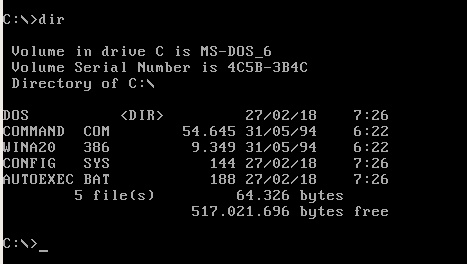
\includegraphics[width=0.68\textwidth]{img/cmd2.png}
        }}
        \subfloat[Ejecución del comando \textit{type}, mostra  contenido archivo. Fallo con autoexec]{\label{fig:sugerencia}{
   		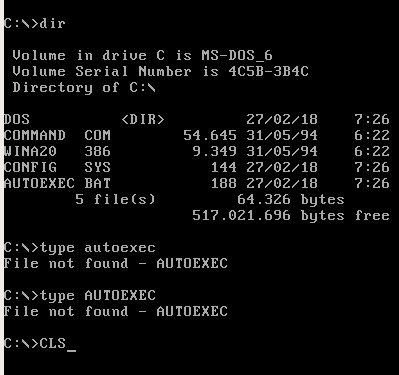
\includegraphics[width=0.68\textwidth]{img/cmd3.png}
        }}
        \hfill
        \subfloat[\textit{cls} limpiar pantalla de Dos]{\label{fig:disponibles}{
   		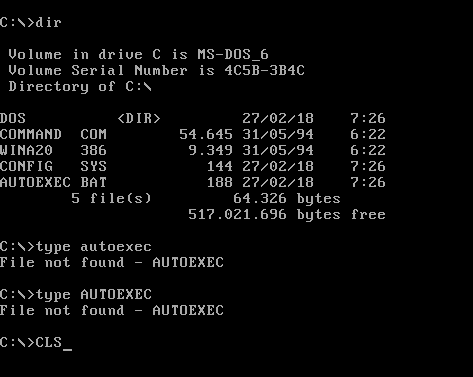
\includegraphics[width=0.64\textwidth]{img/cmd4.png}
        }}
        \subfloat[Creacion de carpetas con \textit{mkdir} ]{\label{fig:sugerencia}{
   		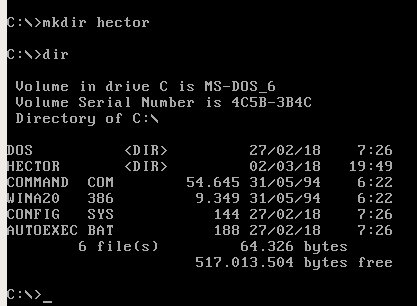
\includegraphics[width=0.64\textwidth]{img/cmd5.png}
        }}
        \hfill
        \subfloat[scandisk, optimizaciones de disco]{\label{fig:disponibles}{
   		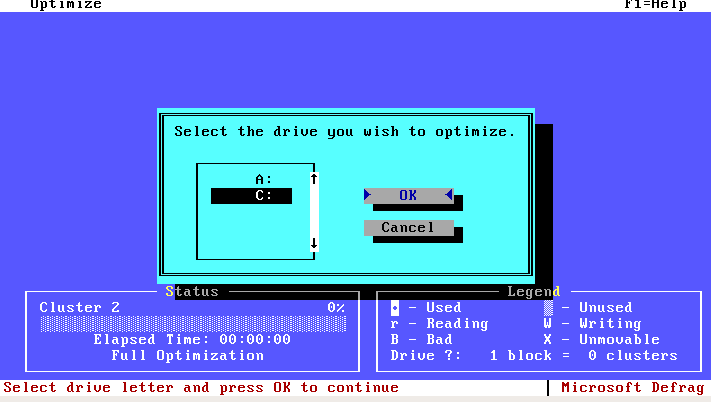
\includegraphics[width=0.68\textwidth]{img/cmd6.png}
        }}
        \subfloat[Desfragmentacion de disco, \textit{defrag c:}]{\label{fig:disponibles}{
   		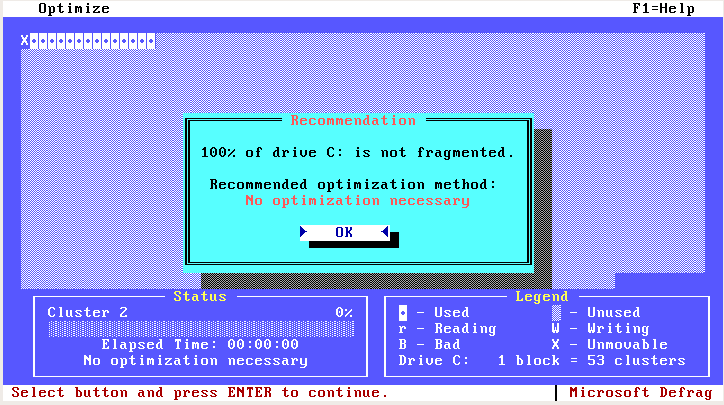
\includegraphics[width=0.68\textwidth]{img/cmd7.png}
        }}
	\caption{Lista de Novedades, Comandos disponibles MSDOS.}
\end{figure}


\begin{figure}[H]
 	\centering
	\subfloat[Ejecución del comando \textit{dir}, listar directorios del sistema]{\label{fig:dircmd}{
   		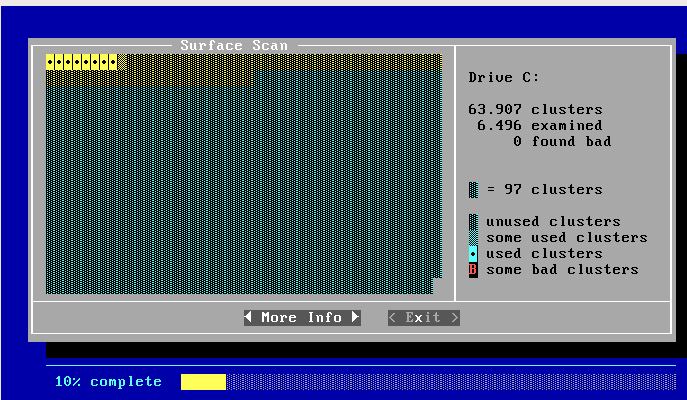
\includegraphics[width=0.68\textwidth]{img/cmd8.png}
        }}
        \subfloat[Ejecución del comando \textit{type}, mostra  contenido archivo. Fallo con autoexec]{\label{fig:sugerencia}{
   		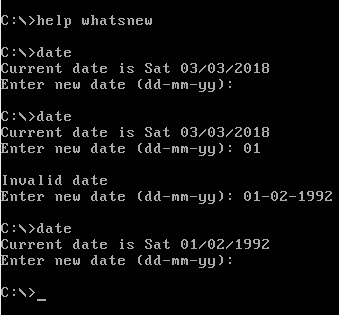
\includegraphics[width=0.68\textwidth]{img/cm9.png}
        }}
        \hfill
        \subfloat[\textit{cls} limpiar pantalla de Dos]{\label{fig:disponibles}{
   		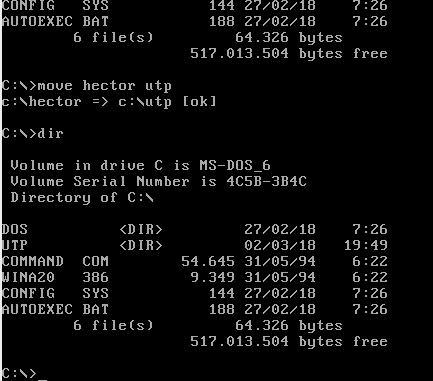
\includegraphics[width=0.64\textwidth]{img/cmd10.png}
        }}
        \subfloat[Creacion de carpetas con \textit{mkdir} ]{\label{fig:sugerencia}{
   		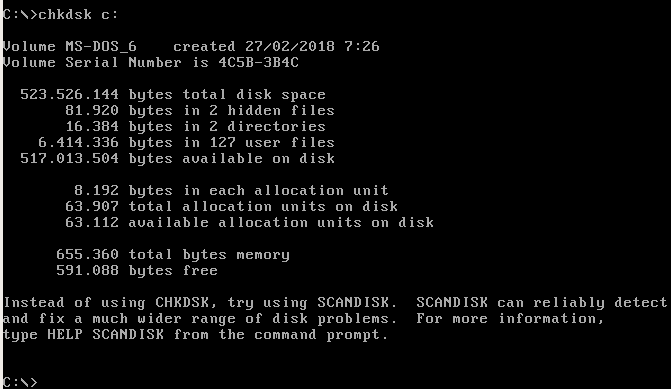
\includegraphics[width=0.64\textwidth]{img/cmd11.png}
        }}
        \hfill
        \subfloat[scandisk, optimizaciones de disco]{\label{fig:disponibles}{
   		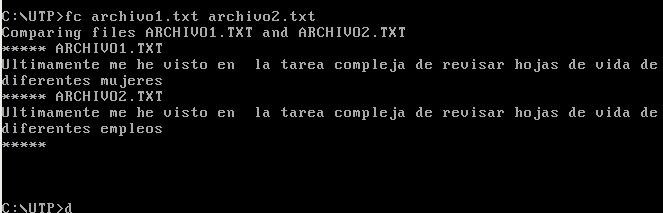
\includegraphics[width=0.68\textwidth]{img/cmd12.png}
        }}
        \subfloat[Desfragmentacion de disco, \textit{defrag c:}]{\label{fig:disponibles}{
   		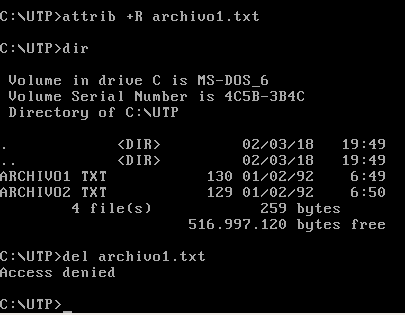
\includegraphics[width=0.68\textwidth]{img/cmd13.png}
        }}
	\caption{Lista de Novedades, Comandos disponibles MSDOS.}
\end{figure}




\section{ Edición de Texto Scripts.}
Para esta sección se conoció de manera directa el editor propio de esta versión de windows6.22.

Toda la informacion para escribir estos programas de QBASIC fueron obtenidas de \fnurl{tedfelix}{http://tedfelix.com/qbasic/}
\begin{figure}[H]
 	\centering
	\subfloat[Puesta a prueba lenguaje QBASIC ]{\label{fig:sugerencia}{
   		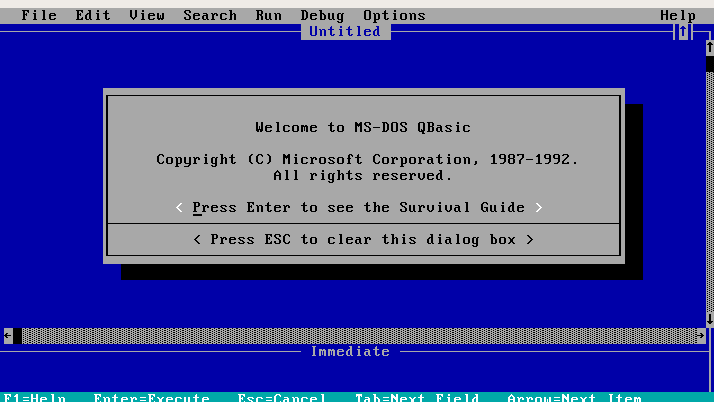
\includegraphics[width=0.68\textwidth]{img/cmd15.png}
        }}
        \subfloat[Puesta a prueba lenguaje QBASIC ]{\label{fig:sugerencia}{
   		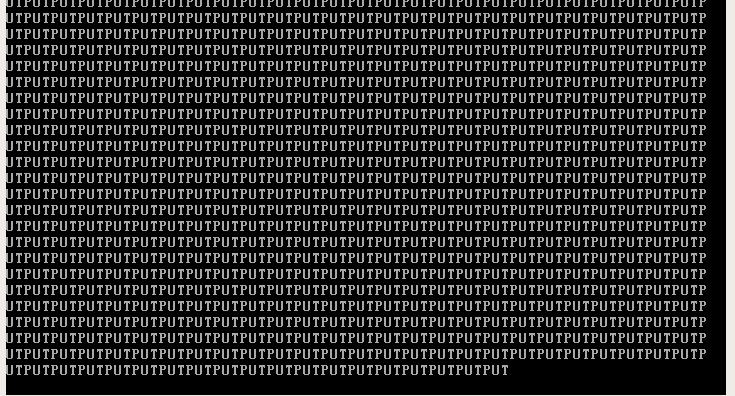
\includegraphics[width=0.68\textwidth]{img/cmd16.png}
        }}
\end{figure}


\begin{figure}[H]
 	\centering
	\subfloat[Escritura en qbasic ]{\label{fig:dircmd}{
   		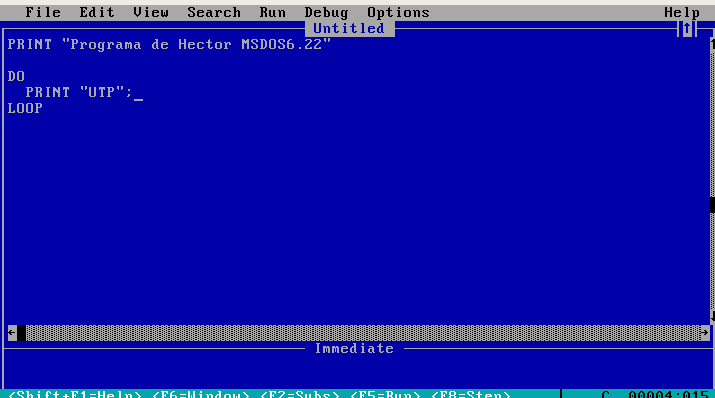
\includegraphics[width=0.68\textwidth]{img/cmd17.png}
        }}
        \subfloat[Ejecución del comando \textit{for}, loop interactivo echo.]{\label{fig:sugerencia}{
   		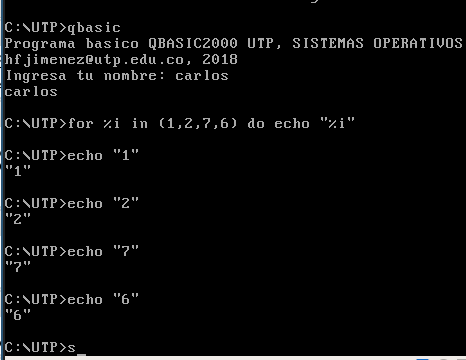
\includegraphics[width=0.68\textwidth]{img/cmd18.png}
        }}
\end{figure}

\section{Referencias}
\begin{itemize}
\item  \hyperref[http://www.instructables.com/id/How-To-Install-DOS-622-Under-VirtualBox/]{DOS Manual Installation,soluciona el error de vídeo,  http://www.instructables.com/id/How-To-Install-DOS-622-Under-VirtualBox/}
\end{itemize}
\end{document}